\documentclass[12pt]{article}
\usepackage{xcolor}
\usepackage[tikz]{bclogo}
\usepackage[framemethod=tikz]{mdframed}
\usepackage{lipsum}
\usepackage[many]{tcolorbox}
\usepackage{ucs}
\usepackage{listings}
\usepackage[utf8x]{inputenc}
\usepackage{hyperref}
\usepackage{amsfonts}
\usepackage{textcomp}
\usepackage{graphicx}
\usepackage{tikz}
\usetikzlibrary{patterns}
\usepackage{pgfplots}
\usepackage{pgfplotstable} 
\usepgfplotslibrary{fillbetween}

\usepackage[printwatermark]{xwatermark}
\newwatermark[allpages,color=gray!15,angle=45,scale=3,xpos=0,ypos=0]{DRAFT}

%To get the bibliography to be listed in the ToC as an unnumbered sectional unit (chapter or section), use tocbibind without the numbib option
\usepackage[nottoc,notlot,notlof]{tocbibind}

\title{Apollo's Scalability}
\date{\today}
\author{Ivan Mamontov}

\pgfplotsset{width=13cm,compat=1.10}


\definecolor{bgblue}{RGB}{245,243,253}
\definecolor{ttblue}{RGB}{91,194,224}


\begin{document}

\maketitle

\tableofcontents{}

\begin{abstract}

This paper characterizes the performance of Apollo on a quite modern Intel\circledR Core\textsuperscript{TM} i7 CPU with Hyper-Threading Technology(HT). Using the performance counters provided by Intel, we quantitatively evaluate micro-architecture metrics while running Apollo. The experimental results reveal that: (1) HT can't improve the performance of Apollo under load; (2) The resource contentions within CPU are the major reason of pipeline inefficiency, which prevents better performance promised by HT; (3) CPU utilization isn't a good estimate of the true load on the system with enabled HT.

\end{abstract}

\section{Theory}

Current trends in microprocessor design have made high resource utilization a key requirement for achieving good performance. For example, while deeper pipelines have led to 3 GHz processors, each new generation of microarchitecture technology comes with increased memory latency and a decrease in relative memory speed. This results in the processor spending a significant amount of time waiting for the memory system to fetch data. This "memory wall" problem continues to remain a major bottleneck\cite{impact}.

Over the years, a number of multithreading techniques have been employed to hide this memory latency. One approach is simultaneous multithreading (SMT), which exposes more parallelism to the processor by fetching and retiring instructions from multiple instruction streams, thereby increasing processor utilization. This allows the CPU to hold the state of different threads and then switch back and forth on a nanosecond time scale. For example, if one of the processes needs to read a word from memory (which takes many clock cycles), a CPU can just switch to another thread. SMT does not offer true parallelism, i.e. only one process at a time is running, but thread-switching time is reduced to the order of a nanosecond\cite{tanenbaum}. Price and performance benefits make SMT a common design choice as, for example, in Intel's Nehalem microarchitecture, where it is called Hyper-Threading (HT) where the physical core contains a mixture of resources, some of which are shared between threads\cite{intel}:

\begin{itemize}
	\item {\em replicated resources} for each thread, such as register state, return stack buffer (RSB), and the instruction queue; 
    \item {\em partitioned resources} tagged by the thread number, such as load buffer, store buffer, and reorder buffer;
    \item {\em shared resources} such as:
    \begin{itemize}
    		\item Istruction fetchers, decoders etc are co-operatively shared between HTs. That is the fetch/decode path alternates between HT threads on each CPU tick. This halves the rate at which instructions can be input at the top of the pipe.
    		\item L1/L2 and TLB space, and for branch prediction resources.
    		\item Reservation Station (RS), where the uops wait until their inputs are available, space in the Reorder Buffer, where the uops wait until they can be retired sufficient load and store buffers in the case of memory related uops
    \end{itemize}
    \item {\em shared resources unaware of the presence of threads}, such as execution units.
\end{itemize}

Because instructions from several threads execute simultaneously, threads compete every cycle for all common hardware resources, such as functional units, instruction queues, renaming registers, caches, and TLBs. Since threads may differ widely in their hardware requirements, some threads may interact poorly when co-scheduled onto the processor. For example, two threads with large cache footprints may cause inter-thread cache misses, leading to low instruction throughput for the machine as a whole. Conversely, threads with complementary resource requirements may coexist on the processor without excessive interference, thereby increasing utilization; for example, integer-intensive and FP-intensive threads should execute well together, since they utilize different functional units. Consequently, thread scheduling decisions have the potential to affect performance, either improving it by co-scheduling threads with complementary hardware requirements, or degrading it by co-scheduling threads with identical hardware needs\cite{smt}.

\section{Practice}

\subsection{Problem definition}

HT can be quite a misleading, for example, if CPU with HT shows 40\% CPU usage, this does not mean that this CPU can handle more than 2 times more work. So when it comes to capacity planning, it's easy to be duped into thinking that CPU utilization is a good estimate of the true load on the system with enabled HT.

\subsection{Experimental platform}

To get a better understanding of how HT impacts performance, consider a single-socket Intel Core i7 processor-based system with four cores (Intel Xeon will have the same result as it uses the same microarchitecture).

\begin{itemize}
	\item {\em OS:} RHEL 7 (kernel 3.10) with CFQ (complete fair queuing) scheduler. 
	\item {\em CPU:} 2.80GHz Intel\circledR Core\textsuperscript{TM} i7 CPU 860 processor with 4 physical cores and 8 hyper-threads. This is a Nehalem - quite old hardware but similar to that used in production.
	\item {\em Memory:} 16GB of dual channel DDR3 memory at 1600MHz.
	\item {\em JVM:} Oracle JDK 1.7.0\_75 with production-like settings.
	\item {\em Apollo:} last stable release with production-like index.
\end{itemize}

\subsection{Benchmark}

Let's assume a jagger\cite{jagger} test which is capable to produce a linearly increasing keyword search load with facets and user filters as in production. There are two cases to check:
\begin{itemize}
	\item HT is disabled, Apollo uses four hardware threads;
	\item HT is enabled, Apollo uses eight software threads;
\end{itemize} 

Figure~\ref{fig:load} shows the results of these experiment. 

\begin{figure}[h]
    \centering
	\begin{tikzpicture}
		\begin{axis}[
			xlabel={Time, s},
			ylabel={Requests per Second},
			grid=major,
			legend entries={Target load, Real load with HT Off, Real load with HT On},
			legend pos=south east,
			xmin=4,xmax=600,
			ymin=0,ymax=30,
		]
		\addplot[dashed,gray,ultra thick,mark=none] coordinates {
			(-10, 0)
      		(90, 5)
     		(190, 10)
      		(290, 15) 
      		(390, 20)
      		(490, 25)
      		(590, 25)
      		(600, 25)
      	};
      	\addplot[blue,very thick,mark=none] table {resources/apollo-search-throughput.csv};
      	\addplot[red,very thick,mark=none] table {resources/apollo-search-throughput2.csv};
		\end{axis}
	\end{tikzpicture}
	\caption{Apollo's throughput with and without HT}
    \label{fig:load}
\end{figure}

\section{Analysis}

\subsection{CPU utilization}

HT has implications for the operating system because each thread appears to the operating system as a separate CPU. So if there is only enough work to keep each hardware thread busy at a certain point in time the operating system will have to place active threads on cores before scheduling on threads on the same core. In other words, up to 50\% of CPU utilization there is almost no difference between HT and non HT CPUs. Figure~\ref{fig:cpu} shows this theory in practice. The results are more than illustrative -- HT does not actually give twice more power in our case. As we can see at 50\% of CPU utilization, the CPU becomes overloaded because the two threads running in the same core are competing for the same resources. If each of the two threads gets only half the amount of a limiting resource then it will run at half speed, and the advantage of HT is completely gone. Two threads running at half speed is certainly not better than a single thread running at full speed.

\begin{figure}[h]
    \centering
	\begin{tikzpicture}
    		\tikzset{
        		hatch distance/.store in=\hatchdistance,
        		hatch distance=10pt,
        		hatch thickness/.store in=\hatchthickness,
        		hatch thickness=2pt
    		}

    		\makeatletter
    		\pgfdeclarepatternformonly[\hatchdistance,\hatchthickness]{flexible hatch}
    		{\pgfqpoint{0pt}{0pt}}
    		{\pgfqpoint{\hatchdistance}{\hatchdistance}}
    		{\pgfpoint{\hatchdistance-1pt}{\hatchdistance-1pt}}%
    		{
        		\pgfsetcolor{\tikz@pattern@color}
        		\pgfsetlinewidth{\hatchthickness}
        		\pgfpathmoveto{\pgfqpoint{0pt}{0pt}}
        		\pgfpathlineto{\pgfqpoint{\hatchdistance}{\hatchdistance}}
        		\pgfusepath{stroke}
    		}

		\begin{axis}[
			xlabel={Time, s},
			ylabel={CPU Utilisation, \%},
			grid=major,
			legend entries={HyperThreading Off,HyperThreading On},
			legend pos=south east,
			xmin=4,xmax=600,
			ymin=0,ymax=100,
		]

		\addplot[blue,very thick,mark=none] table {resources/cpuNehalem.csv};
		\addplot[red,very thick,mark=none] table {resources/cpuNehalem2.csv};
		\addplot[pink,very thin,mark=none,
			pattern=flexible hatch,
    			area legend,
    			pattern color=red,
    			hatch distance=10pt,
        		hatch thickness=0.5pt,
        		draw=red,
		] table {resources/cpuNehalem3.csv}\closedcycle;

		\end{axis}
	\end{tikzpicture}
	\caption{Dependency of the average CPU utilization on linearly increasing keyword search load}
    \label{fig:cpu}
\end{figure}

Unfortunately, sometimes it happens that the operating system lets two threads run in the same processor core, with the other CPU completely idle. This choice is far less efficient than using one thread on each CPU. Figure~\ref{fig:sched} shows this behavior during the test when utilization starts to increase rapidly(red-shaded area on figure~\ref{fig:cpu}). Each horizontal line on this timechart represents logical CPU(from 0 to 7). Each bar on this chart represents a scheduler timeslice. It is obvious that while the first core woks with two threads, "the last core" is idle. It is the responsibility of the operating system to avoid such situations, but unfortunately, in order to avoid unnecessary CPU migrations scheduler decides to keep thread on overloaded core.  

\begin{figure}[h]
    \centering
	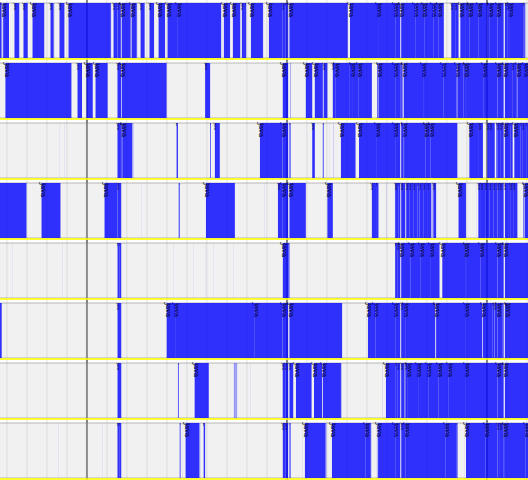
\includegraphics[scale=0.8]{images/scheduler.png}
	\caption{CPU scheduler behavior during the test in the red zone}
    \label{fig:sched}
\end{figure}

\subsection{Analyzing bottlenecks}

In order to better understand the bottleneck it will be useful to use Performance Monitoring Unit (PMU) which is a set of special-purpose registers built into modern microprocessors to store the counts of hardware-related activities such as instruction cycles, cache hits, cache misses, branch misses and many others. Compared to software profilers, hardware counters provide low-overhead access to a wealth of detailed performance information related to CPU's functional units, caches and main memory etc. Another benefit of using them is that no source code modifications are needed in general.

If the performance is limited by any of the shared resources, for example highest-level cache, which is called before accessing memory, is usually referred to as the last level cache(LLC), then the total performance is not increased by HT. Actually, in the worst cases the total performance is decreased by HT because this resources are wasted when the two threads compete for the same resources. Figure~\ref{fig:llc} presents the last level cache misses per 1000 instructions.

\begin{figure}[h]
    \centering
	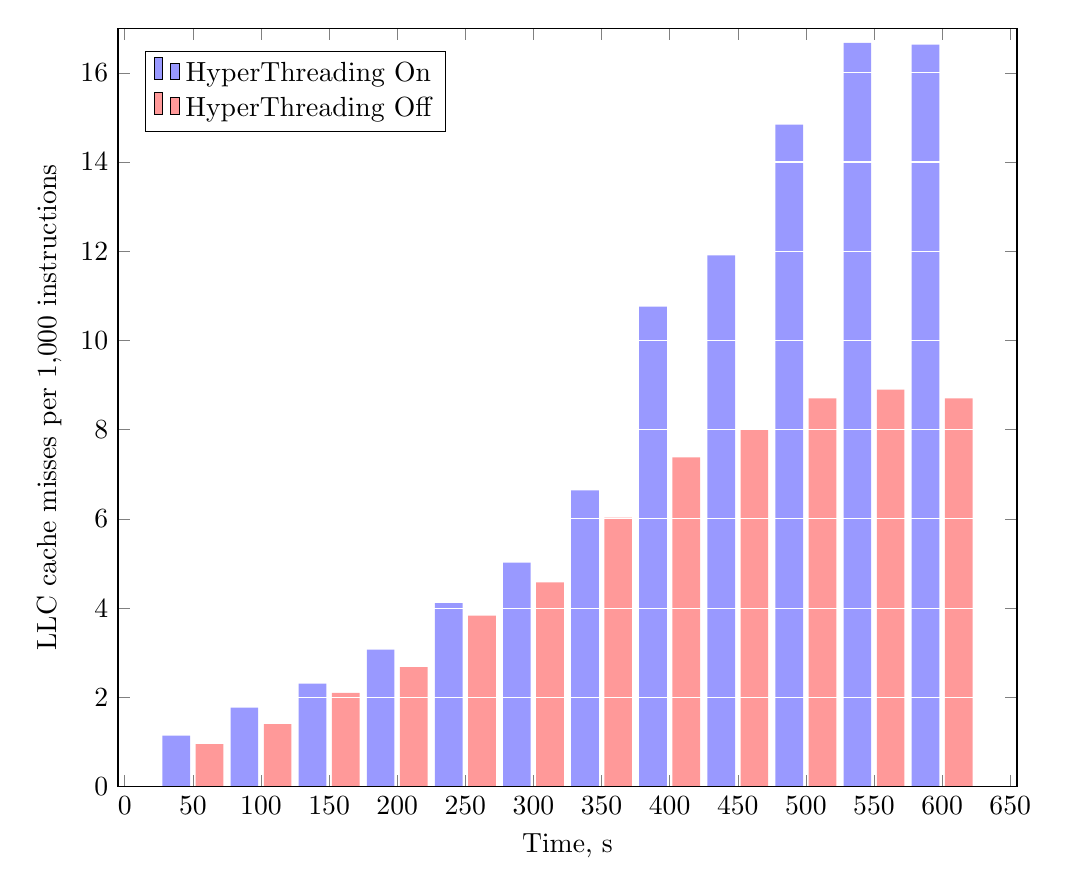
\begin{tikzpicture}
	\begin{axis} [ybar,
			 xlabel={Time, s},
			 ylabel={LLC cache misses per 1,000 instructions},
			 axis on top,
			 ymin=0, ymax=17,
			 xmin=50, xmax=600,
			 legend pos=north west,
			 major grid style={draw=white},
        		 enlarge x limits=true,
        		 ymajorgrids, tick align=inside,
			 ]
	\addplot[draw=none, fill=blue!40] coordinates {
      (50, 1.14)
      (100, 1.77) 
      (150, 2.31)
      (200, 3.07) 
      (250, 4.11) 
      (300, 5.02)
      (350, 6.64) 
      (400, 10.76) 
      (450, 11.91) 
      (500, 14.84) 
	  (550, 16.67) 
      (600, 16.63) };
	\addplot[draw=none,fill=red!40]  coordinates {
      (50,  0.95)
      (100, 1.4) 
      (150, 2.1)
      (200, 2.68) 
      (250, 3.83) 
      (300, 4.58)
      (350, 6.03) 
      (400, 7.38) 
      (450, 8) 
      (500, 8.7) 
	  (550, 8.9) 
      (600, 8.7) };
      \legend{HyperThreading On,HyperThreading Off}
	\end{axis}
	\end{tikzpicture}
	\caption{LLC cache misses per 1,000 instructions}
    \label{fig:llc}
\end{figure}



\begin{verbatim}
      74360.715495   task-clock (msec)         #    3.835 CPUs utilized                                             
    84,400,226,408   stalled-cycles-frontend   #   55.59% frontend cycles idle    
    41,616,239,021   stalled-cycles-backend    #   27.41% backend  cycles idle    
   170,735,558,048   instructions              #    1.12  insns per cycle        
                                               #    0.49  stalled cycles per insn                   
       716,316,970   branch-misses             #    2.33% of all branches         
\end{verbatim}

After ss

\begin{verbatim}
     137014.930439   task-clock (msec)         #    7.839 CPUs utilized                                          
   170,689,428,657   stalled-cycles-frontend   #   70.69% frontend cycles idle    
    47,010,900,540   stalled-cycles-backend    #   19.47% backend  cycles idle    
   187,613,979,340   instructions              #    0.78  insns per cycle        
                                               #    0.91  stalled cycles per insn                
       915,996,259   branch-misses             #    2.70% of all branches         
\end{verbatim}


\section{Conclusion}

Obviously, it can be quite difficult to predict whether HT is good or bad for a particular application. The only safe way of answering this question is to test it. Ideally, we should test our application on several different microprocessors with several different data sets with HT turned on and off.

%Latency is probably always a little worse when HT is on. Throughput may be improved only if you can multithread your workload and that the workload was previously resource limited by something other than CPU execution resources. If CPU resources are the limiting factor, having two independent instruction streams competing for them won't help with either throughput or latency.


%Intel(R) Core(TM) i7 CPU 860 @ 2.80GHz "Intel(r) microarchitecture codename Nehalem/Nehalem-EP"


%\url{http://172.18.128.65:8080/jagger/#metrics?sessions=(ids=514,516)&tests=(name=apollo-search-5-user&trends=stdDevLatency,avgLatency,throughput,CPU%20Load%20Average,CPU%20Utilization)}
%\url{http://www.cs.washington.edu/research/smt/papers/threadScheduling.pdf}
%The default process scheduler in Linux (as of kernel 2.6.34) is CFQ (Completely Fair Queuing).

%\renewcommand\bcStyleTitre[1]{\large\textcolor{ttblue}{#1}}
%\begin{bclogo}[
%  couleur=bgblue,
%  arrondi=0,
%  logo=\bclampe,
%  barre=none,
%  noborder=true]{Quiz}
%How many minor GC cycles are shown on the Figure~\ref{fig:sched}?
%\end{bclogo}


\begin{thebibliography}{1}

  \bibitem{impact} Subhash Saini, Haoqiang Jin {\em The Impact of Hyper-Threading on Processor Resource Utilization in Production Applications}

  \bibitem{tanenbaum} Andrew S. Tanenbaum {\em Modern Operating Systems. Fourth Edition}

  \bibitem{intel} David Levinthal {\em Performance Analysis Guide for Intel® Core™ i7 Processor and Intel® Xeon™ 5500 processors} \url{https://software.intel.com/sites/products/collateral/hpc/vtune/performance_analysis_guide.pdf}
  
  \bibitem{smt} Sujay Parekh, Susan Eggers {\em Thread-Sensitive Scheduling for SMT Processors}
  
  \bibitem{agner} Agner {\em Fog How good is hyperthreading?} Available at \url{http://agner.org/optimize/blog/read.php?i=6}

  \bibitem{jagger} \url{https://jagger.griddynamics.net/}
  
  \bibitem{intel2} Garrett Drysdale, Antonio C. Valles, Matt Gillespie {\em Performance Insights to Intel® Hyper-Threading Technology}
  
  \bibitem{} Wei Huang, Jiang Lin, Zhao Zhang, J. Morris Chang{\em Performance Characterization of Java Applications on SMT Processors}
  
  \bibitem{vtune} Intel Corp. {\em VTune performance analyzer.} Available at \url{http://www.intel.com/software/products/vtune/}
  
  \bibitem{intel3} Intel Corp. {\em Intel® 64 and IA-32 Architectures Optimization Reference Manual} \url{http://www.intel.com/content/www/us/en/architecture-and-technology/64-ia-32-architectures-optimization-manual.html}

  \bibitem{gregg} Brendan D. Gregg {\em Active Benchmarking} http://www.brendangregg.com/activebenchmarking.html
  
  \bibitem{perf} \url{https://perf.wiki.kernel.org/index.php/Main_Page}

\end{thebibliography}

\end{document}


